
In this chapter we will take a closer look at random walks, both in general and the transition from the statistical view to partial differential equations. 
We will take a look at different algorithms to produce random walks, and discuss their pros and cons in light of this project. 
Then we will take a quick look at partial differential equations and numerical solution of them.

\section{Introduction to random walks}\label{introduction_to_random_walks}
The most basic random walk is a walker on the x-axis which will take a step of a fixed length to the right with a probability $p$, or to the left with a probability $q=1-p$. 
Using (pseudo-) random numbers on a computer we can simulate the outcomes of a random walk. 
For each step (of which there are N) we draw a random number, r, between 0 and 1 from some distribution (say a uniform one) which will be the probability. 
If $r\leq p$ the walker will take a step to the left, otherwise it will take a step to the right. 
After the N steps the walker will have taken R steps to the right, and $L = N-R$ steps to the left. 
The net displacement from the origin will be $S = R-L$. \\
This simple approach is easily generalizable to two and three dimensions by having $2d$ possible outcomes from the random number, where d is the dimensionality. 
In two dimensions the walker will step up if $r\in(0.75,1]$ and left if $r\in[0,0.25)$, for example.

\subsection{Further discussion and analysis of the introduction}\label{further_introduction}
The following derivation is borrowed from a compendium in statistical mechanics by Finn Ravndal. \\
If we do sufficiently many walks, the net displacement will vary from $S=+N$ to $S=-N$ representing all steps to the right and all steps to the left respectively. 
The probability of all steps being to the right is $P_N(N) = p^N$. 
Should one of the steps be to the left, and the rest to the right we will get a net displacement of $S = N-2$ with the probability $P_N(R = N-1) = Np^{N-1}q$. 
We can generalize this to finding the probability of a walk with a R steps to the right as 
\begin{equation}\label{bernoulli_distr}
 P_N(R) = {N\choose R}p^{R}q^{N-R}
\end{equation}
where ${N\choose R}=\frac{N!}{R!(N-R)!}$ is the number of walks which satisfy the net displacement in question, or the multiplicity of this walk in statistical mechanics terms. 
Equation \ref{bernoulli_distr} is the Bernoulli probability distribution, which is normalized.
\begin{align*}
 \sum\limits_{R=0}^N P_N(R) = (p+q)^N = 1^N = 1
\end{align*}
We can use this distribution to calculate various average properties of a walk consisting of N steps. 
For example, the average number of steps to the right is
\begin{align*}
 \langle R\rangle &=  \sum\limits_{R=0}^N RP_N(R) =  \sum\limits_{R=0}^N {N\choose R}Rp^Rq^{N-R} = \\
 p\frac{d}{dp} \sum\limits_{R=0}^N {N\choose R}p^Rq^{N-R} &= p\frac{d}{dp}(p+q)^N = Np(p+q)^{N-1} = Np
\end{align*}
From this we can also find the average value of the net displacement using $S = R-L = R-(N-R) = 2R-N$.
\begin{align*}
 \langle S\rangle = \langle2R\rangle -N = 2Np-N(p+q) = N(2p-p-q) = N(p-q)
\end{align*}
We notice that the average net displacement is greatly dependent on the relationship between $p$ and $q$, and that any symmetric walk will have an expected net displacement of zero. 
In many cases we will be more interested in the mean square displacement than the displacement itself, because many important large scale parameters can be related to the root-mean-square displacement. 
This can also be calculated rather straightforwardly. 
\begin{align*}
  \langle R^2\rangle =  \sum\limits_{R=0}^N R^2P_N(R) &=  \sum\limits_{R=0}^N {N\choose R}R^2p^Rq^{N-R} = \\
 \left(p\frac{d}{dp}\right)^2 \sum\limits_{R=0}^N {N\choose R}p^Rq^{N-R} &= \left(p\frac{d}{dp}\right)^2(p+q)^N \\
 = Np(p+q)^{N-1} +p^2N(N-1)(p+q)^{N-2} &= (Np)^2 +Np(1-p) = (Np)^2 +Npq
\end{align*}
Like before, the average net displacement is given as $S^2 = (2R-N)^2$ and we obtain
\begin{align*}
 \langle S^2\rangle = 4\langle R^2\rangle -4N\langle R\rangle + N^2 &= 4((Np)^2 +Npq) -4N^2p + N^2\\
 = N^2(4p^2 -4p +1) +4Npq &= N^2(2p-1)^2 +4Npq = N^2(p-q)^2 +4Npq.
\end{align*}
which for the 1D symmetric walk gives $\langle S^2\rangle =N$ and the variance, denoted $\langle\Delta S^2\rangle = \langle\langle S^2\rangle-\langle S\rangle^2\rangle$, is found by insertion as
\begin{align}
 \langle\Delta S^2\rangle &= \langle N^2(p-q)^2 +4Npq - ( N(p-q))^2\rangle= 4Npq 
\end{align}
<<<<<<< HEAD
When the number of steps gets very large we can approximate the Bernoulli distribution \ref{bernoulli_distr} by the Gaussian distribution. 
=======
When the number of steps gets very large we can approximate the Bernoulli distribution (eq. \ref{bernoulli_distr}) by the Gaussian distribution. 
>>>>>>> 5c5037ade39e1aacd97e655ab856f7981aebbe61
This is most easily done in the symmetric case where $p=q=\frac{1}{2}$, but it is sufficient for the steplengths to have a finite variance (\emph{find something to refer to}). 
The Bernoulli distribution then simplifies to
\begin{equation}
 P(S,N) = \left(\frac{1}{2}\right)^N\frac{N!}{R!L!}
\end{equation}
<<<<<<< HEAD
on which we apply Stirling's famous formula for large factorials $n!\simeq\sqrt{2\pi n}n^ne^{-n}$.
=======
on which we apply Stirling's famous formula for large factorials $n!\simeq\sqrt{2\pi n}\cdot n^ne^{-n}$.
>>>>>>> 5c5037ade39e1aacd97e655ab856f7981aebbe61
\begin{align*}
 P(S,N) &= \left(\frac{1}{2}\right)^N\frac{N!}{R!L!} \\
 &= \exp\left(-N\ln2+\ln\sqrt{2\pi N}+N\ln N - \ln\sqrt{2\pi R} -R\ln R - \ln\sqrt{2\pi L} - L\ln L \right) \\
 &= \sqrt{\frac{N}{2\pi RL}}\exp\left(-R\ln\frac{2R}{N}-L\ln\frac{2L}{N}\right)
\end{align*}
Where we have used $R+L=N$. We now insert for $\frac{2R}{N}=1+\frac{S}{N}$ and $\frac{2L}{N}=1-\frac{S}{N}$ and expand the logarithms to first order, $RL=\frac{N^2-S^2}{4}$ in the prefactor, and approximate $1-\frac{S^2}{N^2}\simeq1$. This gives
\begin{equation}\label{descrete_gaussian_distr}
 P(S,N) =\sqrt{\frac{2}{\pi N}}\exp\left(\frac{-S^2}{2N}\right)
\end{equation}
which is an ordinary, discrete Gaussian distribution with $\langle S\rangle = 0$  and $\langle S^2\rangle = N$. 
If we keep assuming that the walker is on the x-axis, and let the step length, a, get small the final position will be $x=Sa$ which we can assume is a continuous variable. 
Similarly, we let the time interval between each step, $\tau$, be small and let the walk run for a continuous time $t=N\tau$. This changes the distribution \ref{descrete_gaussian_distr} to
\begin{equation}
 P(x,t) = \frac{1}{2a}\sqrt{\frac{2\tau}{\pi t}}\exp\left(-\frac{x^2\tau}{2a^2t}\right). 
\end{equation}
The prefactor $\frac{1}{2a}$ is needed to normalize the continuous probability distribution since the separation between each possible final position in walks with the same number of steps is $\Delta x=2a$. 
We also introduce the diffusion constant
\begin{equation}
D = \frac{a^2}{2\tau} 
\end{equation}
making the distribution
\begin{equation}
 P(x,t) = \sqrt{\frac{1}{4\pi Dt}}\exp\left(-\frac{x^2}{4Dt}\right)
\end{equation}
<<<<<<< HEAD
Introducing $x$ also gives us the expected value and variance of x on a form which will be useful later. 
=======
Introducing $x$ also gives us the expectation value and variance of x on a form which will be useful later. 
>>>>>>> 5c5037ade39e1aacd97e655ab856f7981aebbe61
We have $x=Sa$ which means 
$$\langle x\rangle=a\langle S\rangle$$ 
and 
$$\langle x^2\rangle=a^2\langle S^2\rangle$$
Finally by insertion we find the variance $\langle \Delta x^2\rangle$
\begin{equation}\label{random_walk_variance}
 \langle \Delta x^2\rangle = \langle\langle x^2\rangle -\langle x\rangle^2\rangle = \langle a^2\langle S^2\rangle -a^2\langle S\rangle^2\rangle = 4Npqa^2
\end{equation}


\subsection{More general Random Walks}\label{more_general_random_walks}

In the more general case, the position of a random walker,$\vec{r}$ at a time $t_i$ is given by the sum
\begin{equation}\label{brownian_motion}
 \vec{r}(t_i)=\sum\limits_{j=0}^i \Delta \vec{x}(t_j)
\end{equation}
where $\Delta \vec{x}(t_j) = \left(\Delta x(t_j),\Delta y(t_j),\Delta z(t_j)\right)$ in 3D. Each $\Delta x,\Delta y,\Delta z$ is a random number drawn from a distribution with a finite variance $\sigma^2 = \langle\Delta x^2\rangle$. 
By the central limit theorem, any stochastic process with a well defined mean and variance can, given enough samples, be approximated by a Gaussian distribution. 
This means that the probability of finding the walker at some position x after M steps is 
\begin{equation}
 P(x,M)\propto e^{-\frac{x^2}{2M\sigma^2}}
\end{equation}
Remember that the actual Gaussian distribution is 
$$
\frac{1}{\sqrt{2\pi\sigma^2}}\exp\left(\frac{(n-\mu)^2}{2\sigma^2}\right)
$$
<<<<<<< HEAD
We can introduce an Einstein relation $\sigma^2 = 2D\Delta t$ and the obvious relation $t = M\Delta t$ to get a more desirable exponent.
We see that $\langle \Delta x^2\rangle = 2Dt$. 
=======
We can introduce an Einstein relation $\sigma^2 = 2dD\Delta t$ and the obvious relation $t = M\Delta t$ to get a more desirable exponent.
We see that $\langle \Delta x^2\rangle = 2Dt$ in the one dimensional case where $d=1$. 
>>>>>>> 5c5037ade39e1aacd97e655ab856f7981aebbe61
\emph{The introduction of the Einstein relation might put some restrictions on our model.}
Normalizing the expression gives us 
\begin{equation}\label{rw_gaussian_distribution}
 P(x,t) = \sqrt{\frac{1}{4Dt}}\exp\left(-\frac{x^2}{4Dt}\right)
\end{equation}

If we have a large number, N, of walkers, their concentration will be $C(x,t) = NP(x,t)$. 
The concentration is conserved, so any amount that flows out of an area must reflect as a decrease in concentration. 
We can express this by the flow of concentration
\begin{equation}
 \frac{\d C}{\d t} -\nabla\cdot\vec{J} = S
\end{equation}
where $\vec{J}$ is the flow vector and S is a source term which in our case will be zero.
From Fick's first law we know that $\vec{J} = -D\nabla C$. Inserting this gives us
\begin{equation}\label{simple_diffusion_equation}
 \frac{\d C}{\d t} = \nabla\cdot \left(D\cdot\nabla C\right)
\end{equation}
which is the diffusion equation.
By insertion we can check that this version (\ref{rw_gaussian_distribution}) of the Gaussian distribution fulfills the diffusion equation. 
Starting with only the time derivative gives us
\begin{align*}
 \frac{\d P}{\d t} = -\frac{4\pi D\exp\left(-\frac{x^2}{4Dt}\right)}{2\sqrt{(4\pi Dt)^3}}&+\frac{x^2\exp\left(-\frac{x^2}{4Dt}\right)}{4Dt^2\sqrt{4\pi Dt}} \\
 = \exp\left(-\frac{x^2}{4Dt}\right)\left(\frac{8Dx^2}{2\sqrt{\pi}(4Dt)^{5/2}} -\frac{(4D)^2t}{2\sqrt{\pi}(4Dt)^{5/2}}\right)&= \frac{4D\exp\left(-\frac{x^2}{4Dt}\right)(x^2-2Dt)}{\sqrt{\pi}(4Dt)^{5/2}}
\end{align*}
 We then finish by doing the spatial derivative
\begin{align*}
 D\frac{\d^2 P}{\d x^2} &= \frac{D}{\sqrt{4\pi Dt}}\frac{\d}{\d x}\left[-\exp\left(\frac{-x^2}{4Dt}\right)\left(\frac{-2x}{4Dt}\right)\right]\\
 = \frac{2D}{4Dt\sqrt{4\pi Dt}}&\exp\left(\frac{-x^2}{4Dt}\right)\left[1-x\left(\frac{2x}{4Dt}\right)\right] = \frac{4D\exp\left(-\frac{x^2}{4Dt}\right)(x^2-2Dt)}{\sqrt{\pi}(4Dt)^{5/2}}
\end{align*}
and see that they are equal, meaning that the diffusion equation is satisfied.

\subsection{Choosing random walk algorithm}\label{choosing_random_walk_algorithm}

As this article points out \cite{farnell2005monte} the simplest random walk model, which places walkers on discrete mesh points and uses a fixed step length, has been used with great success to model diffusion processes. 
<<<<<<< HEAD
However, this model will struggle with reproducing anisotropic diffusion, that is $D = D(x)$. Farnell and Gibson also suggest a method for improving the results by adjusting the step length according to position, thus effectively adjusting the diffusion constant of the walk as well. 
=======
However, this model will struggle with reproducing anisotropic diffusion, that is $D = D(x)$. Farnell and Gibson also suggest a method for improving the results by adjusting the step length and probability according to position, thus effectively adjusting the diffusion constant of the walk as well. 
>>>>>>> 5c5037ade39e1aacd97e655ab856f7981aebbe61
We see then that the simplest model is rather robust, and well tested. 
However, the aim of this project is to combine two realistic models for diffusion on different length scales, and the simplest random walk model has one fundamental flaw in that view; it is not a realistic model for diffusing particles. 
Brownian motion is a more realistic physical model for diffusing particles, and can (I think) quite easily be modified to model anisotropic diffusion as well. 
We can model Brownian motion simply by using equation \ref{brownian_motion}, and we can with a bit of work expand it to model collisions between walkers as well. \\
That being said, by the central limit theorem both models will after some timesteps be described by a Gaussian distribution meaning that on the PDE scale we will not know the difference. 
Hence it will make no sense to not use the simplest random walk model.


\subsection{Random walks and anisotropy}\label{random_walks_and_anisotropy}

Any real problem where parts of the diffusion process cannot be modelled by the continuum approximation is bound to be anisotropic. 
There is reason to believe that an anisotropic diffusion process on the PDE level will lead to an anisotropic random walk model as well, but how do we model this. 
Equation \ref{steplength} shows the step length as a function of the diffusion constant. 
If we simply replace the diffusion constant by a function $D = D(\vec{x})$ we are at least started, but this will not quite be sufficient as Farnell and Gibson point out \cite{farnell2005monte}. 
Through their experiments they found that only adjusting the steplength will not improve the error noticeably and reasoned that this is because the walkers are still as likely to jump in both directions (right or left in 1d), and that the stepsize is the same in both cases, hence the model does not resemble anisotropy. 
They went on to introduce an adjusted steplength and an adjusted step probability, a solution they landed on after trial and error. 
The expressions they proposed are listed in equations \ref{farnell_and_gibson_1} to \ref{farnell_and_gibson_5}. 
\begin{equation}\label{farnell_and_gibson_1}
 \Delta_p(x) = \frac{1}{2}\left(L(x) + L(x +\Delta_p(x))\right) \to L(x) +\frac{1}{2}L(x)L'(x)
\end{equation}
\begin{equation}\label{farnell_and_gibson_2}
 \Delta_m(x) = \frac{1}{2}\left(L(x) + L(x -\Delta_m(x))\right) \to L(x) +\frac{1}{2}L(x)L'(x)
\end{equation}
where $L(x)$ is defined in equation \ref{farnell_and_gibson_3} and $\Delta_p(x)$ and $\Delta_m(x)$ are the adjusted steplengths to the right and left, respectively.
\begin{equation}\label{farnell_and_gibson_3}
L(x) = \sqrt{2D(x)\Delta t}
\end{equation}
We also have the adjusted jump probabilities $T_r(x)$ and $T_l(x)$ which are the probabilities for a walker in position x to jump right or left, respectively. 
These are defined in equations \ref{farnell_and_gibson_4} and \ref{farnell_and_gibson_5}
\begin{equation}\label{farnell_and_gibson_4}
T_r(x) = \frac{1}{2} +\frac{1}{4}L'(x)
\end{equation}
\begin{equation}\label{farnell_and_gibson_5}
T_l(x) = \frac{1}{2} -\frac{1}{4}L'(x)
\end{equation}
We notice that the adjusted steplength we proposed to start with is still a part of the final expressions.


\subsection{Random walks and drift}\label{random_walks_and_drift}

Another point we have yet to say something about is diffusion that has a drift term, $\frac{\d u}{\d x}$. 
<<<<<<< HEAD
Initially one thought that diffusion in the ECS of the brain was governed by a drift term , but the modern perception is that this drift term is in the very least negligible \cite{nicholson2001diffusion}.
=======
Initially one thought that diffusion in the Extra Cellular Space of the brain was governed by a drift term, but the modern perception is that this drift term is in the very least negligible \cite{nicholson2001diffusion}.
>>>>>>> 5c5037ade39e1aacd97e655ab856f7981aebbe61
The drift term might be of importance in other applications, however, and something we should look into it.\\
How do we model random walks with drift? \\
A first instinct is to simply add some vector to the Brownian motion model, thus forcing all walkers to have a tendency to walk a certain direction. 
This approach can also be used in the fixed steplength (or variable steplength in the anisotropic case)  if we express the new step, $\vec{s}$, as
\begin{align*}
 \vec{s} = (\pm l \text{ or }0,\pm l \text{ or }0) +\vec{d}
\end{align*}
where $\vec{d}$ denotes the drift of the walker.\\
We can set up the continuity equation for a concentration, $C(x,t) = NP(x,t)$ of random walkers which are affected by a drift.
\begin{equation}
 \frac{\d C}{\d t} +\nabla\cdot\vec{j} = S
\end{equation}
Where $\vec{j}$ denotes the total flux of walkers through some enclosed volume and $S$ is a source/sink term. 
Since the walkers are affected by drift the flux will consist of two terms; $\vec{j} = \vec{j}_{diff}+\vec{j}_{drift}$. 
From Fick's first law we know that $\vec{j}_{diff} = -D\nabla C$. 
The second flux term is the advective flux which will be equal to the average velocity of the system; $\vec{j}_{drift} = \vec{v}C$. 
Inserting this in the continuity equation gives us the well known convection diffusion equation (\ref{convection_diffusion_equation}).
\begin{equation}\label{convection_diffusion_equation}
 \frac{\d C}{\d t} = \nabla\cdot\left(D\nabla C\right)-\nabla\cdot\left(\vec{v}C\right) + S
\end{equation}
Which in many cases will simplify to
\begin{equation}
 \frac{\d C}{\d t} = D\nabla^2 C-\vec{v}\cdot\nabla C
\end{equation}

In order to determine all the parameters of the convection diffusion equation \ref{convection_diffusion_equation} we will need to go through some of the calculations from chapter \ref{introduction_to_random_walks}. 
The situation is the same, a walker in one dimension which can jump left or right, but this time will also move a finite distance $d$ each timestep. 
This will make the expected net displacement
\begin{equation*}
 \langle S\rangle = R-L +Nd = N(p-q) + Nd
\end{equation*}
and the expected mean square displacement
\begin{equation*}
 \langle S^2\rangle = (2\langle R\rangle -N)^2 +(Nd)^2 = N^2(p-q)^2 +4Npq +(Nd)^2
\end{equation*}
which in turn gives us the variance
\begin{align*}
 \langle \Delta S^2\rangle &= \langle\langle S^2\rangle-\langle S\rangle^2\rangle \\
 &= N^2(p-q)^2 +4Npq +(Nd)^2 - N^2(p-q)^2 -(Nd)^2 \\
\langle \Delta S^2\rangle &= 4Npq
\end{align*}
This shows us that the variance is untouched by the drift term, but not the mean which for the symmetric case is $\langle S\rangle = Nd$. 
When we convert this to the continuous variables $x$ and $t$ we get the solution shown in equation \ref{solution_convection_diffusion_eq}.
\begin{equation}\label{solution_convection_diffusion_eq}
 C(x,t) = \frac{N}{\sqrt{4\pi Dt}}\exp\left(-\frac{(x-vt)^2}{4Dt}\right)
\end{equation}
Where $v = \frac{d}{\Delta t}$ is the velocity of the concentration and $D$ is the well known diffusion constant, inserted from the Einstein relation $\sigma^2 = 2D\Delta t$.\\
The only problem with the solution \ref{solution_convection_diffusion_eq} is that it is invalid for $t=0$. 
In order to use it we will need an initial condition which fits the rest of the solution. 
We try and find this by first checking by simulation if it converges towards some initial solution as $t\to0$ and if so, extrapolate this to $t=0$ as the initial condition. 
Figure \ref{convection_diffusion_eq_initial_condition} shows the result of this little experiment, and as we clearly see it does diverge as $t\to0$. 
However, it also converges to a Dirac delta function, $\delta(x)$ which is defined by its properties
\begin{align*}
\delta(x) = \begin{cases} +\infty, & x = 0 \\ 0, & x \ne 0 \end{cases}
\end{align*}
and
\begin{equation*}
 \int_{-\infty}^\infty \delta(x) \, dx = 1
\end{equation*}
The Dirac delta function often sought as an initial condition in experimental setups for measurements on diffusion processes because of its compatibility with a variety of diffusion equations, and should do a very good job in our numerical setup as well. 

\begin{figure}[H]
 \centering
 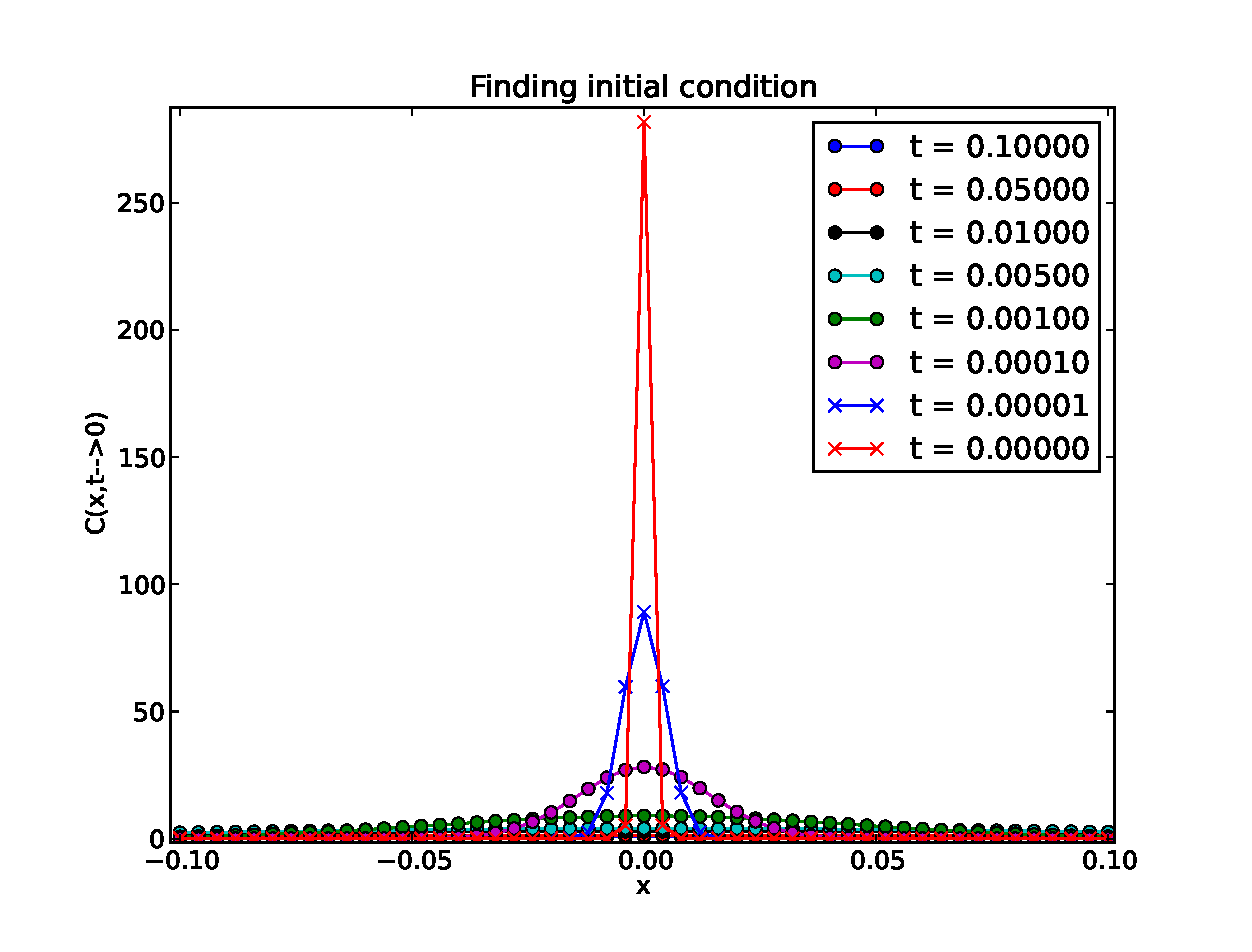
\includegraphics[scale=0.7]{Figures/convection_diffusion_eq_initial_condition.eps}
 \caption[Initial condition for convection diffusion]{Experiment to determine the initial condition of equation \ref{solution_convection_diffusion_eq}}
 \label{convection_diffusion_eq_initial_condition}
\end{figure}


\section{Some words about partial differential equations}\label{some_words_on_PDEs}
\subsection{Discretizing}\label{discretizing}

To maintain a bit of generality we will look at the (potentially) anisotropic diffusion equation in 2d. The extension to 3d is trivial, as is the 1d version.
\begin{equation}
 \frac{\d u}{\d t} = \nabla D\nabla u +f
\end{equation}
where f is some source term. 
The final expression and scheme will depend on how we chose to approximate the time derivative, but the spatial derivative will mostly have the same approximation. \\
We start off by doing the innermost derivative in one dimension. 
The generalization to more dimensions is trivial, and will consist of adding the same terms for the y and z derivatives. 
\begin{align*}
 \left[\frac{d}{dx}u\right]^n \approx \frac{u^n_{i+1/2}-u^n_{i-1/2}}{\Delta x}
\end{align*}
Where we have made the approximate derivative around the point $x_i$. 
We then set $\phi(x)=D\frac{du}{dx}$ and do the second derivative
\begin{align*}
  \left[\frac{d}{dx}\phi\right]^n \approx \frac{\phi^n_{i+1/2}-\phi^n_{i-1/2}}{\Delta x}
\end{align*}
and insert for $\phi$
\begin{align*}
 \frac{\phi^n_{i+1/2}-\phi^n_{i-1/2}}{\Delta x} = \frac{1}{\Delta x^2}\left(D_{i+1/2}(u^n_{i+1}-u^n_{i+1}) -D_{i-1/2}(u^n_{i}-u^n_{i-1})\right)
\end{align*}
Since we can only evaluate the diffusion constant at the mesh points (or strictly speaking since it is a lot simpler to do so) we must approximate $D_{i\pm1/2}\approx0.5(D_{i\pm1}+D_i)$. 
Inserting this gives us 
\begin{align*}
 \nabla D\nabla u\approx\frac{1}{2\Delta x^2}\left((D_{i+1,j}+D_{i,j})(u_{i+1,j}-u_{i,j})-(D_{i,j}+D_{i-1,j})(u_{i,j}-u_{i-1,j})\right) \\
 +\frac{1}{2\Delta y^2}\left((D_{i,j+1}+D_{i,j})(u_{i,j+1}-u_{i,j})-(D_{i,j}+D_{i,j-1})(u_{i,j}-u_{i,j-1})\right)
\end{align*}
The Forward Euler discretization has one drawback which is its instability for ``large'' $\Delta t$. 
A common tradeoff for explicit numerical schemes. 
We could sacrifice ease of implementation for unconditional stability in our scheme. 
At least in 1d the implementation is not that much worse either if we chose the Backward Euler discretization for an isotropic (homogeneous) equation. 
The discretization itself is found in equation \ref{BE_discretisation_isotropic}. 
\begin{equation}\label{BE_discretisation_isotropic}
 \frac{u^n_i - u^{n-1}_i}{\Delta t} = D\frac{u^n_{i+1}-2u^n_i +u^n_{i-1}}{\Delta x^2}
\end{equation}
The advantage of this discretization is that it results in a tridiagonal linear system, which we can easily find if we just insert the first couple of steps.
\begin{align*}
 \frac{u^{n}_i-u^{n-1}_i}{\Delta t} = D\frac{u^n_{i+1}-2u^n_i + u^n_{i-1}}{\Delta x^2} \\
 u^n_i -\frac{D\Delta t}{\Delta x^2}\left(u^n_{i+1}-2u^n_i + u^n_{i-1}\right) = u^{n-1}_i \\
 u^n_i\Big(1+2\dfrac{D\Delta t}{\Delta x^2}\Big) -u^n_{i-1}\dfrac{D\Delta t}{\Delta x^2} - u^n_{n+1}\dfrac{D\Delta t}{\Delta x^2} 
 = u^{n-1}_i
\end{align*}
If we insert for a few steps we see that this takes the form of
\begin{align*}\label{BE}
 \left(\begin{array}{c c c c c c c c}
        \Big(1+2\alpha\Big) & -\alpha &0 &\dots & & &0 &0 \\
        -\alpha & \Big(1+2\alpha\Big) & -\alpha &0 &\dots & & &0 \\
        0& \ddots & \ddots & \ddots & 0 & \dots &  &0\\
        0& \dots & & &0&-\alpha & \Big(1+2\alpha\Big) & -\alpha\\
         0& \dots & && &0&-\alpha & \Big(1+2\alpha\Big) 
       \end{array}\right)\mathbf{u}^n = \mathbf{u}^{n-1} 
\end{align*}
where we have set $\alpha = \frac{\Delta t}{D\Delta x^2}$.
\begin{equation*}
 \mathbf{A}\mathbf{u}^n = \mathbf{u}^{n-1}
\end{equation*}
This can be solved very efficiently by a sparse Gaussian elimination, which is quite simple to implement once you take the boundary conditions into account. 
We implement the Backward Euler discretization in order to efficiently simulate for longer times, and by extension to test the effects the longer time steps will have on the random walk model. More on the tridiagonal Gaussian elimination in the appendix.\\
We would, of course, also like an implicit solver in 2 and 3d as well to make sure that we can take longer time steps here as well. 
Doing the BE discretization in 2d gives us a slightly more difficult linear problem (eq \ref{linear_system_BE2D}), which is still sparse, but we do not have any simple, efficient solver for five-band matrices. 
Further difficulties arise when we attempt to implement Neumann boundary conditions of girds larger than $3\times3$ since the off-diagonal elements do not ``hit'' their intended matrix-elements. 
In order to use the 2D BE scheme we must either invert a cubic matrix and multiply it by a normal matrix, or we will have to start rearranging the elements in the vectors (converted matrices) and the entries in the linear-problem matrix correspondingly. 
All things considered, we will therefore try and find another implicit scheme for our 2D problem. 
There is another discretization which lets us utilize our tridiagonal solver, and is implicit and unconditionally stable in 2d, the Alternate Direction Implicit (ADI) scheme. 
The ADI scheme divides the time step in two and only propagates one of the spatial derivatives at a time, making it very similar to the Crank Nicholson scheme. 
In fact, the truncation error in the ADI scheme is of second order, just as in the CN scheme, but this is (as discussed earlier) of small importance in this thesis. 
Discretizing the simple diffusion equation by the ADI scheme is done as follows.
\begin{align*}
 \frac{u^{n+1/2}-u^n}{\Delta t/2} &= D\left(D_xD_xu^{n+1/2}+D_yD_yu^n\right)\\
 \frac{u^{n+1}-u^{n+1/2}}{\Delta t/2} &= D\left(D_xD_xu^{n+1/2}+D_yD_yu^{n+1}\right)
\end{align*}
We can write this as two standard equations on the form 
\begin{align*}
\mathbf{A}_{1/2}\mathbf{u}^{n+1/2} = \mathbf{u}^n \\
\mathbf{A}_{1}\mathbf{u}^{n+1} = \mathbf{u}^{n+1/2} 
\end{align*}
Note that the indices are only intended as labels. For a $3\times3$ mesh the equations are shown in the appendix.\\
After more careful calculations, we find that the ADI discretization does not, in fact, produce a tridiagonal linear problem when we introduce the Neumann boundary conditions. 
While the scheme is still a viable alternative for other applications, considering its second order convergence, there is no benefit in using it for our application and we can concentrate on the normal Backward Euler discretization using a pre-exisiting solver for the linear problem as a first approach. \\
As an improvement we note that the Matrix in the linear problem stays the same as long as $\Delta t$ is unchanged. This means that we can get away with assembling the matrix once, and it lets us do an LU decomposition which will reduce the number of FLOPS needed per time-step from $\mathcal{O}(N^3)$ to $\mathcal{O}(N^2)$ where $N$ is the product of the number of mesh-points in x and y direction. 
In other words, since we have chosen the same resolution in x and y direction (and the time dependence can be related to this resolution as well for the explicit schemes) if we chose a resolution of $n$ we will need $n^4$ FLOPS per time-step as opposed to the $n^2$ for the explicit scheme.




\subsection{Stability}\label{stability}

In section \ref{discretizing} we used the Forward Euler approximation to the time derivative. 
Unfortunately the resulting scheme is potentially unstable, as we shall now see. 
We start out by assuming that the solution $u(x,t)$ is on the form 
\begin{equation}\label{von_neumann_fourier_solution}
 u(x,t) = A^n\exp(ikp\Delta x)
\end{equation}
where $i^2=-1$ is the imaginary unit and $A^n$ is an amplification factor which, for the solution \ref{von_neumann_fourier_solution} ideally should be $\exp(-\pi^2t)$, but will be something else in the numerical case. 
We notice that we must have $\left|A\right|\leq 1$ if $u$ is to not blow up. 
Inserting \ref{von_neumann_fourier_solution} in the simplified version of the variable coefficient scheme (where the coefficient is constant) gives us the following
\begin{align*}
 \exp(ikp\Delta x)\left(A^{n+1}-A^n\right) &= A^n\frac{D\Delta t}{\Delta x^2}\left(\exp(ik(p+1)\Delta x)-2\exp(ikp\Delta x) +\exp(ik(p-1)\Delta x)\right)\\
  A^n\exp(ikp\Delta x)\left(A-1\right) &=  A^n\exp(ikp\Delta x)\frac{D\Delta t}{\Delta x^2}\left(\exp(ik\Delta x) -2 + \exp(-ik\Delta x)\right)\\
\end{align*}
Using the well known identities $\exp(iax)+\exp(-iax) = \frac{1}{2}\cos^2\left(\frac{ax}{2}\right)$  and $\cos^2(ax)-1 = \sin^2(ax)$ gives us
\begin{equation}
 A-1 = \frac{D\Delta t}{\Delta x^2}\sin^2\left(\frac{k\Delta x}{2}\right)
\end{equation}
We now insert for the ``worst case scenario'' $max(\sin^2\left(\frac{k\Delta x}{2}\right))= 1$
\begin{equation}
 A = \frac{D\Delta t}{2\Delta x^2}+1 \implies \Delta t\leq\frac{\Delta x^2}{2D}
\end{equation}
In 2d this criterion is halved, and for the anisotropic case we must insert for the maximum value of D which, again, will be the ``worst case scenario''.\\
If we insert the same solution (eq. \ref{von_neumann_fourier_solution}) in the BE scheme we get
\begin{align*}
 \exp(ikp\Delta x)\left(A^{n}-A^{n-1}\right) &= A^n\frac{D\Delta t}{\Delta x^2}\left(\exp(ik(p+1)\Delta x)-2\exp(ikp\Delta x) +\exp(ik(p-1)\Delta x)\right)\\
  A^n\exp(ikp\Delta x)\left(1-A^{-1}\right) &=  A^n\exp(ikp\Delta x)\frac{D\Delta t}{\Delta x^2}\left(\exp(ik\Delta x) -2 + \exp(-ik\Delta x)\right)\\
\end{align*}
which leads to 
\begin{equation}\label{stability_BE}
A = \frac{1}{ 1+\frac{D\Delta t}{\Delta x^2}}
\end{equation}
Equation \ref{stability_BE} is smaller than 1 for all $\Delta t>0$ which means that the scheme is unconditionally stable.

\subsection{Truncation error}\label{truncation_error}

As we know the numerical derivative is not the analytical derivative, but an approximation. 
This approximation has a well defined residual, or truncation error which we can find by Taylor expansion.
\begin{equation*}
  R = \frac{u(t_{n+1}) -u(t_n)}{\Delta t} -u'(t_n)
\end{equation*}
Remember Taylor expansion of $u(t+h) = \sum\limits_{i=0}^\infty\frac{1}{i!}\frac{d^i}{dt^i}u(t)h^i$
\begin{align*}
 R &= \frac{u(t_n)+u'(t_n)\Delta t +0.5u''(t_n)\Delta t^2 + \mathcal{O}(\Delta t^3)-u(t_n)}{\Delta t} -u'(t_n)\\
  &= u''(t_n)\Delta t+ \mathcal{O}(\Delta t^2) = \mathcal{O}(\Delta t)
\end{align*}
We can do better than this by using another discretization scheme for the PDE, but in our case the PDE is not the only error source seeing as we will combine it with a random walk solver. 
Quantifying an error term for the random walk solver is not straightforward, but naturally it will be closely coupled to the number of walkers used. 
So far the error seems to behave as expected, meaning that introducing very many walkers might reduce the error to $\mathcal{O}(\Delta t^2)$ if the number of walkers, $N$ is proportionate to $N\propto\frac{1}{\Delta t^2}$. 
Since $\Delta t \leq\frac{D\Delta x^2}{2}$ by the stability constraint (in 1D), we will already for small meshes of some 20 points need to introduce $\sim600000$ walkers per unit ``concentration'' per meshpoint in the walk-area. 
This will be such a costly operation that it will not necessarily be worth it.\\
The spatial derivative also has a well defined residual which is found by Taylor expansion.
\begin{equation}
R = \frac{u(x_{i+1})-2u(x_i)+u(x_{i-1})}{\Delta x^2}-u''(x_i) 
\end{equation}
Remember Taylor expansion of $u(x-h) = \sum\limits_{i=0}^\infty\frac{1}{i!}\frac{d^i}{dt^i}u(x)(-h)^i$
\begin{align*}
 R &= \frac{u(x_i)+u'(x_i)\Delta x +0.5u''(x_i)\Delta x^2 + \frac{1}{6}u^{(3)}(x_i)\Delta x^3) +\frac{1}{24}u^{(4)}(x_i)\Delta x^4 +\mathcal{O}(\Delta x^5)}{\Delta x^2}-\frac{2u(x_i)}{\Delta x^2}+\\
 &\frac{u(x_i)-u'(x_i)\Delta x +0.5u''(x_i)\Delta x^2 - \frac{1}{6}u^{(3)}(x_i)\Delta x^3) +\frac{1}{24}u^{(4)}(x_i)\Delta x^4 +\mathcal{O}(\Delta x^5)}{\Delta x^2} -u'(x_i)\\
R &= u''(x_i) +\frac{1}{12}u^{(4)}(x_i)\Delta x^2 + \mathcal{O}(\Delta x^5)  -u''(x_i) = \mathcal{O}(\Delta x^2) 
\end{align*}
There are discretizations that can reduce this residual even further (although a second order scheme is usually considered adequate), but this time the stability criterion on the time derivative \ref{stability} will always be of the order $\mathcal{O}(\Delta x^2)$ and so we will never get a smaller error than this unless we change the time derivative.


\section{Combining the two solvers}\label{combining_the_solvers}
This section will deal with the actual combination of the two models.\\

\subsection{The basic algorithm}\label{basic_algorithm}

The basic structure of the program is to have one solver-object which contains one PDE-solver for the normal diffusion equation, and a linked list of random walk-solvers and their relevant areas. 
Before we start we must add an initial condition along with some parameters such as the diffusion constant (/tensor) and $\Delta t$, and we have the opportunity to mark areas on the mesh where we want random walk solvers. 
The method for adding walk-areas will map them to an index and set the initial condition for the walk. 
In the future we plan to add the possibility of setting boundary conditions and having anisotropy follow into the random walk solvers as well.
At each timestep we call the solve-method of the combined solver, which in turn calls the solve method for the PDE-solver. 
We then loop over the random walk solvers and call their solve-methods. 
The results of these are inserted in the solution from the PDE using some routine (e.g. the average of the two) and the timestep is done. 
A schematic of the algorithm is provided in figure \ref{schematic}.

\begin{figure}[H]
\centering
% \includegraphics{schematic.eps}
\caption[Algorithm]{Schematic diagram of the algorithm.}
\label{schematic}
\end{figure}
section
\subsection{Potential problems or pitfalls with combining solutions}\label{problems_and_pitfalls}

There are a few obvious difficulties we can expect to run into in our planned project. 
Future ones will be added here as well.

\begin{itemize}
 \item Different timescales\\
  The PDE-solver will be operating with some timestep $\Delta t$ which will, depending on the discretization of the PDE, have some constraints and will definitely have an impact on the error. 
  The walkers will, as we have just seen, solve the diffusion equation as well, but with some different $\Delta \tilde{t}$ which is smaller than the timestep on the PDE level. 
  Depending on the coupling chosen between the two models this difference will have some effect or a catastrophic effect on the error. 
  Running some number of steps, N, on the random-walk level should eventually sum up to the timestep on the PDE level, $\sum\limits_{i=0}^N \Delta\tilde{t} = \Delta t$. 
  It turns out, as we will see in section \ref{probability_distribution_and_timesteps} that we can make sure the coupling is as good as it gets by restricting the step length of the walkers.
 \item Boundary conditions\\
 To combine the two models we will need to put restricting boundary conditions on the random walks. This is not usually done (as far as I have seen), but not very difficult. 
 Finding a boundary condition that accurately models the actual system turns out to be quite straightforward, so long as the walk-domain is not on the actual boundary of the whole system. 
 We can assume that the number of walkers in the walk-domain is conserved for each PDE-timestep, and thus no walkers can escape the domain. 
 Implementing perfectly reflecting boundaries solves this quite well. 
 This means that the flux of walkers out of a boundary is zero, which is the same as Neumann boundary conditions on the PDE level. \\
 Dirichlet boundaries can (probably) be implemented by adding or removing walkers on the boundaries (or in a buffer-zone around them) until we have the desired concentration of walkers.
 \item Negative concentration of walkers \\
 The concentration of walkers is calculated as $NP(x,t)$ where $P(x,t)$ is really only an estimate of the actual probability distribution, calculated by dividing the number of walkers in one area $x\pm\frac{\Delta x}{2}$ by the total number of walkers. 
 Seeing as negative probabilities does not make sense, and neither does a negative number of walkers, we will eventually run into some problems when the solution of the PDE takes negative values (which it might do). 
 The solution to this is simply to store the signs of the solution to the PDE in an array, and send only positive values to the random walk solver. 
 When we convert the number of walkers back to a PDE solution we still have the sign from before and can multiply the concentration by the sign it had in the last timestep. 
 \item Smooth solutions\\
 A diffusion process is very effective when it comes to dampening fast fluctuations, and so any solution of the diffusion equation will be smooth. 
 When we introduce a stochastic process, we will potentially also introduce fast fluctuations from one timestep to the next. 
 In this case we are faced with a dilemma; on the one hand there is the smoothness of the solution to consider, on the other hand we have introduced the stochastic term believing that it adds detail to our model. 
 The approach we use to this is to do some curve-fitting using both of the solutions. 
 This will give us some difference between the two models and some smoothness.
 \item Number of timesteps on the random walk level\\
 As the timestep on the PDE level is increased above the stability criterion of the FE scheme towards more efficient sizes we are faced with the problem of whether or not to increase the number of timesteps on the RW level. 
 Strictly speaking we do not have to do this, seeing as we adjust the steplength of the walkers with respect to the timestep (see eq \ref{steplength}). 
 As an initial value we put the number of timesteps to 100, but this was more a guess of how many are necessary for the central limit theorem to have effect than anything else. 
 The question really boils down to how we define our model, which we have yet to do in an accurate way.
 \item Random walks in 3D\\
 Both 1 and 2 dimensional space are spanned completely by a random walk, but space of 3 or more dimensions is not. 
 This does not have to be a problem, seeing as we have proved that the random walk fulfills the diffusion equation (chapter \ref{more_general_random_walks}) and we are not trying to span the complete 3d space, but we could potentially meet some difficulties as a result of this property of the random walk.
\end{itemize}

\subsection{Probability distribution and timesteps}\label{probability_distribution_and_timesteps}
As we saw in section \ref{more_general_random_walks} the probability of finding a walker at a position $x_i$ after some $N$ timesteps (on the walk-scale) is (in the limit of large $N$) given as the Gaussian distribution. 
In our application, however, we are not interested in finding the walker at an exact position, but in an interval around the mesh-points sent to the walk-solver. 
This interval is (for obvious reasons) $x_i\pm\frac{\Delta x}{2}$ where $\Delta x$ is the mesh resolution on the PDE level. 
We will also run the walk solver for some $N$ timesteps on the random-walk scale (where $N$ steps on the random walk scale is the same as one step on the PDE scale). 
This slightly modifies our distribution into
\begin{equation}
 P(x_i\pm\Delta x,t_{n+1}) = \frac{1}{\sqrt{4\pi DN\Delta \tilde{t}}}\exp\left(\frac{(x\pm\Delta x)^2}{4DN\Delta \tilde{t}}\right)
\end{equation}
This makes the concentration of walkers $C(x,t) = MP(x,t)$
\begin{equation}
 C(x_i\pm\Delta x,t_{n+1}) = \frac{M}{\sqrt{4\pi DN\Delta \tilde{t}}}\exp\left(\frac{(x\pm\Delta x)^2}{4DN\Delta \tilde{t}}\right)
\end{equation}
For each PDE-timestep we reset the walkers to have some new initial condition. 
We do this because the concentration over the ``walk-area'' will change with each PDE-timestep.
The point is that $ C(x_i\pm\Delta x,t_{n+1})$ will be dependent on the initial condition $ C(x_i\pm\Delta x,t_{n})$.


Looking at the difference in timestep size between the two length scales we see from equation \ref{descrete_gaussian_distr} that the stepsize on the random walk scale is dependent on the variance in the actual steps (This is in principle the Einstein relation). 
\begin{equation}
 \sigma^2 = \langle\Delta x^2\rangle = 2DN\Delta\tilde{t} \implies \Delta\tilde{t} = \frac{\langle\Delta x^2\rangle}{2DN}
\end{equation}
Equating this with \ref{random_walk_variance} gives us a first order approximation to the steplength, $l$
\begin{align}
 \langle\Delta x^2\rangle &= 4pqNl^2 = 2DN\Delta\tilde{t} \nonumber \\ 
 l &= \sqrt{2D\Delta\tilde{t}}. \label{steplength}
\end{align}
Of course this is assuming that we use a random walk algorithm of fixed steplength.